\section{Resultados}

\subsection{Ruta 1 (www.u-tokyo.ac.jp)}

La primera ruta estudiada fue la que lleva al sitio de la
universidad de Tokyo de Japón (\textsc{UTokyo}). La dirección \texttt{URL} de la
misma es \emph{http://www.u-tokyo.ac.jp} que al momento de realizar el
experimento resolvía a la dirección \texttt{IP} \texttt{210.152.135.17}. Este
destino es de particular interés por su lejanía geográfica.

Habiendo ejecutado la herramienta desarrollada, se obtuvo una ruta que llega al
destino con $\texttt{TTL} = 22$.

\begin{figure}[H]
    \figdef[dim]{figures/tokyo_route_table}
    \caption{Dirección \texttt{IP} para cada \texttt{TTL}.}
\end{figure}

De los $22$ paquetes enviados, $4$ de ellos no generaron
respuesta, lo cual representa un $18$\% de los saltos en la ruta. Ignorando
estos puntos para los cuales no fue posible obtener información, la trayectoria
obtenida tiene una longitud de $18$ saltos.

Como se puede observar en la Figura \ref{res:esc1:map}, hay un total de 3 saltos
intercontinentales. Para confirmar este hecho se buscó la geolocalización de las
direcciones \texttt{IP} involucradas en diversos sitios que prestan este
servicio y efectivamente corresponden a los países señalados.

\begin{figure*}
    \figdef[dim]{figures/tokyo_route_map}
    \caption{Localización de saltos según geolocalización de direcciones IP para
    el sitio \emph{www.u-tokyo.ac.jp}.}
    \label{res:esc1:map}
\end{figure*}

Esto es de particular interés puesto que la comunicación podría haberse
realizado yendo directo a Estados Unidos y luego a Japón, sin embargo, todas las
veces que se observó la trayectoria, la misma contenía el salto a Europa.

Con respecto a los resultados obtenidos mediante el método \emph{Cimbala}, se
pueden observar varias cuestiones. El mismo detecta como \emph{outliers} los
saltos $11$ (\texttt{129.250.2.227}) y $14$ (\texttt{129.250.3.86}). El salto
$11$ efectivamente corresponde al intercontinental de Europa a Estados Unidos.
Por otro lado, el $14$ es perteneciente y le sigue una dirección de Estados Unidos,
con lo cual resulta extraño el hecho de que figure como \emph{outlier}. Sumado a
esto está el hecho de que el resto de los saltos intercontinentales no fueron
detectados.

Un valor sumamente importante para analizar por qué se obtuvieron tales
resultados es el \texttt{RTT} promedio entre saltos. Para este destino en
particular llaman la atención los siguientes puntos:

\begin{itemize}
    \item Tiempo nulo entre saltos
    \item Tiempo muy bajo entre saltos intercontinentales
\end{itemize}

Para los tiempos nulos entre saltos existen varias explicaciones posibles. Al
medir el tiempo que tomaban en ir y volver los mensajes se observó que en
algunos casos al incrementar el \texttt{TTL}, el paquete tardaba menos. Esto lo
que genera es que al querer tomar la diferencia de tiempo entre estos puntos se
obtenga un resultado negativo. Para evitar esto y poder aplicar el método de
\emph{Cimbala} se tomó la decisión de asignarles un valor nulo. Ahora, que los
paquetes \emph{tarden menos} puede ser consecuencia de diversos factores. Uno es
que el camino por el cual viaja la respuesta del \texttt{ICMP} no tiene por qué
ser el mismo que por el utilizado para llegar al destino.  Esto significa que con un
\texttt{TTL} mayor podría suceder que el mensaje vuelva por un camino menos
congestionado bajando así su \texttt{RTT} al punto donde resulta menor que el
del nodo anterior. Otra posible explicación es la del balanceo de carga, donde
puede ocurrir que para los distintos valores de \texttt{TTL} el paquete enviado
no tenga el mismo recorrido.

El tiempo bajo para saltos intercontinentales también resulta llamativo y podría
explicarse también como el resultado de estar tomando las diferencias de tiempo
sobre valores que no reflejan correctamente las rutas reales. Con $\texttt{TTL}
= 17$ (\texttt{61.200.80.218}) se debería estar midiendo el tiempo del salto
intercontinental de Estados Unidos a Japón, sin embargo en la tabla se puede
observar que la diferencia de tiempo es prácticamente nula. Muy posiblemente lo
que esté ocurriendo en este caso particular es que el valor medido para el
\texttt{TTL} anterior corresponda a una ruta distinta a la que termina siendo
utilizada para el salto intercontinental.


\subsection{Ruta 2 (www.mpg.de)}

Luego estudiamos dos rutas distintas para llegar desde Argentina a la página web de los Institutos Max Planck (\texttt{www.mpg.de}), en Alemania. Al momento de realizar los experimentos, la IP a la que resuelve ese host es \texttt{134.76.31.198}. Elegimos este destino para hacer una comparación que nos parecía interesante: rutas a través de proveedores comerciales de Internet, y rutas a través de redes académicas como RedClara y Géant. Para hacer la comparación, ejecutamos la herramienta desde la red de la FCEyN y desde Fibertel, en ambos casos, conectados por Ethernet a cada red.

\subsubsection{Ruta 2A - Internet comercial}

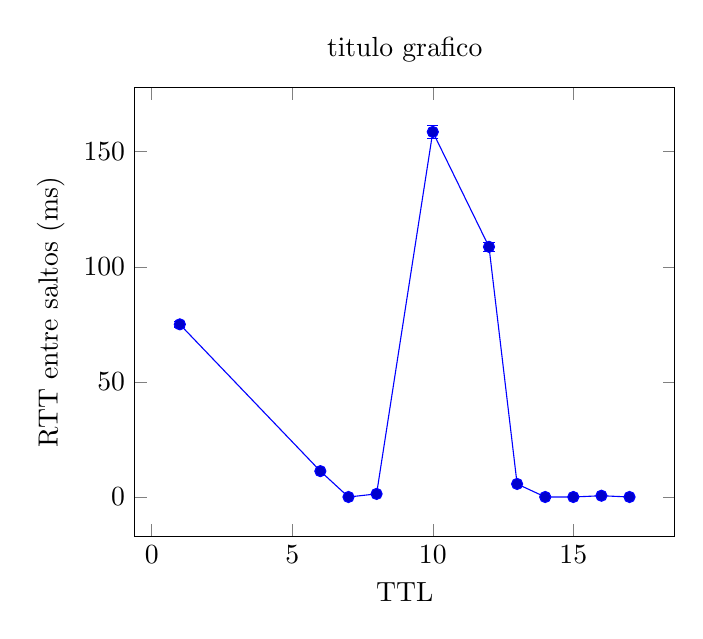
\begin{tikzpicture}
  \begin{axis}[
    title=titulo grafico,
    ylabel=RTT entre saltos (ms),
    xlabel=TTL
  ]
    \addplot+[error bars/.cd,
    y dir=both,y explicit]
    coordinates {
    (1,75)     +- (0,1.13)
    (6,11.23)  +- (0,0.24)
    (7,0)      +- (0,0.5)
    (8,1.34)   +- (0,0.45)
    (10, 158.6)  +- (0,2.9)
    (12,108.67)  +- (0,1.84)
    (13, 5.67)   +- (0,0.36)
    (14,0)       +-  (0,0.74)
    (15,0)       +-  (0,0.8)
    (16,0.55)    +-  (0,0.47)
    (17,0)       +-  (0,0.51)
    };
  \end{axis}
\end{tikzpicture}